\newcommand{\dedx}{$\mathrm d E / \mathrm d x$ }
\chapter{Momentum estimation of slow pions with the ADC in the VXD}

When looking onto the typical momentum distribution of the particles flying through the tracking detectors as show in figure \ref{fig-particles-momentum} it is clear that there is a significant amount of so called slow pions with momenta below $\unit[120]{MeV}$. These particles get produced at the interaction point but because of their small momentum and therefore high curvature and their huge energy losses they can not be detected in the CDC tracking detector. This means they can only be measured in the VXD. Because of the small radius of the VXD and the resulting small number of independent measurement points, the momentum resolution is very poor as it can be seen also in the Glückstern formula
\begin{align*}
 \frac{\sigma_{p_T}}{p_T} = \sqrt{\frac{720}{N + 4}} \sigma_x \frac{p_T \text{[GeV]}}{0.3 q B \text{[T]} L^2}
\end{align*}
where L is the length of the track in the detector and $N$ is the number of measurement points. Decreasing the magnetic field would increase the curvature of the low momentum pions and would therefore make them detectable in the CDC also increasing the number of measurement points. But this would also make the resolution of the high momentum particles very poor. In this thesis a different approach is chosen. Together with the measured positions an independent momentum estimation based on the energy loss per length of the particles is introduced and used in the trajectory fit after the track finding. These added measurements bias the fit towards the correct momentum and can therefore help to increase the momentum resolution.

\begin{figure}
 \centering
 %\includegraphics[width=0.6\linewidth]{figures/vxd/momentumDistriution.pdf}
 \todo{missing figure}
 \caption{Momentum distribution split by different particle types as generated by the simulation. As this simulation is modeled after the physical branching fractions the here shown distribution is also the expected observation in the experiment.}
 \label{fig-particles-momentum}
\end{figure}

As it was shown in previous studies \cite{robert}, the momentum resolution compared to the result of the helix fit with the positions only can be increased by using the information from the energy loss of all hits in the track together. In the quoted paper an advanced summation was used to build a mean energy loss of the slow pions which was transformed to a momentum by a precalculated formula. This momentum estimation was then compared to the one coming from the helix fit. To increase the resolution even more the two different approaches are combined in the presented algorithm.

In figure \ref{fig-dedx-over-p} the energy loss per travel length in the VXD sensors for low momentum pions is shown. How these numbers are calculated is described in the next sections. As it can be seen the \dedx increases with falling momentum of the particles. This relation can be also seen in the already quoted Bethe formula \ref{form-bethe} in chapter \ref{chapter-ex} which can be reduced to 
\begin{align*}
 -\left \langle \dd{E}{x} \right\rangle \approx \frac{4 \pi n z^2}{m_e v^2} \left( \frac{e^2}{4 \pi \varepsilon_0} \right)^2 \ln \left( \frac{2 m_e v^2}{I} \right)
\end{align*} \todo{see in chapter 1: described mean?}
for small particle energies. The equation can be used to calculate the momentum with the energy loss per travel length. But as this formula describes the averaged energy loss it is only correct for all small number of cases. The variance in the energy loss is distributed according to a landau distribution which is described later in more detail. This deviation from the Bethe formula decreases the momentum resolution of the estimation based on the energy loss.

\begin{figure}
 \centering
 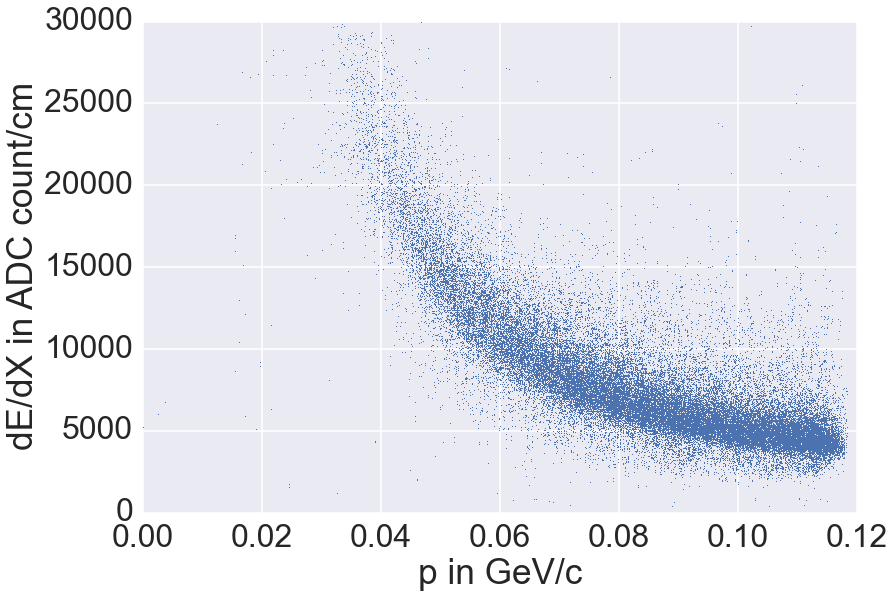
\includegraphics[width=0.8\linewidth]{figures/vxd/dedx.png}
 \todo{Bethe fomrular einfügen!}
 \caption{\dedx information of the VXD clusters of approximately 100000 pions in the momentum range from 50 to 120 MeV. The averaged energy loss can be described by the Bethe formula. The distribution of energy losses for a given momentum is distributed according to a landau distribution which is described later in mroe detail.}
 \label{fig-dedx-over-p}
\end{figure}


\section{Prestudies on the distribution of dE/dX in the VXD}

For the following studies an event sample of slow pions in the momentum range between $\unit[50]{MeV}$ and $\unit[120]{MeV}$ is used. It is simulated using the particle gun with 10 particles per event evenly distributed among the momentum range and between the two charge modes. Different event sampled where used for testing and fitting. The standalone VXD track finder or the MC track finder for reference is used to create tracks out of the simulated VXD hits. As the finding efficiency of the standalone VXD track finder depends heavily on the momenta of the particles, the distribution of the found tracks is not flat any more as it can be seen in figure \ref{fig-vxd-finding-efficiency}. A typical event display can be seen in picture \ref{fig-vxd-event-display}.

\begin{figure}
 \centering
 \caption{Momentum distribution of the simulated pions as found by the VXD track finder and the MC track finder (which has the simulated truth information). The finding efficiency decreases with lower momenta as the number of hits in the VXD is lower for slow pions and the energy loss is stronger. The MC track finder has also not a flat distribution of momenta as it only uses those particles for tracks which have at least 3 hits in the VXD detector.}
 \label{fig-vxd-finding-efficiency}
\end{figure}

\begin{figure}
 \centering
 \caption{Typical event display of one event used for analyzing the momentum estimation for the fitting procedure in the helix fit.}
 \label{fig-vxd-event-display}
\end{figure}

Before calculating the function to transform the \dedx to a momentum estimation and using this information in the helix fit some prestudies are performed to check for the consistency of the input data. They are shown here for reference too.

For calculating the path length used in the \dedx value the correct position of the hit and the sensor information is needed. This information is provided by the clusters used in the track finder. Its results can be seen in figure \ref{fig-cluster-position} where the distance to the beam pipe over the z position is shown for some SVD hits. This position is later used to calculate the path length of the tracks in the sensor region.

\begin{figure}
 \centering
 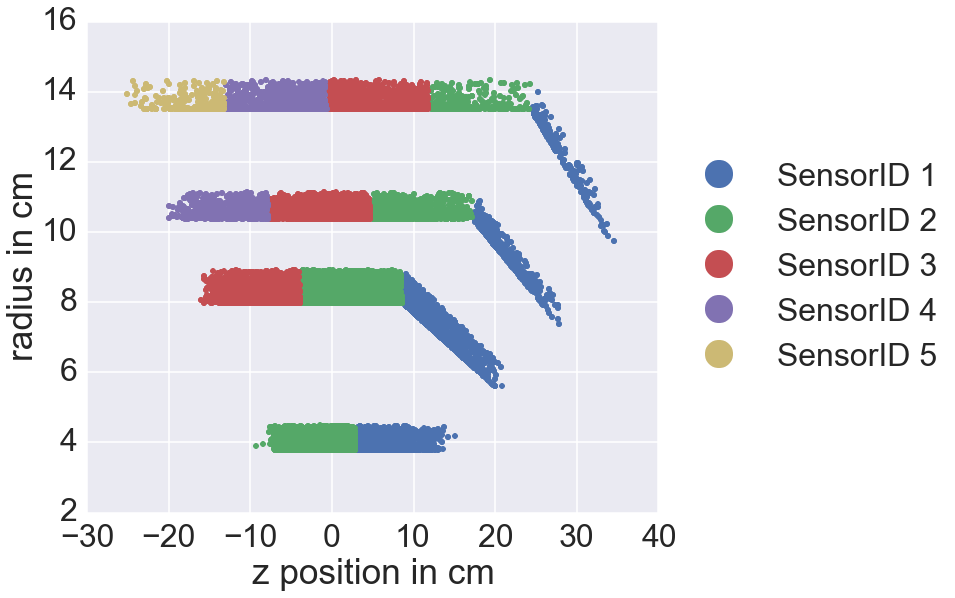
\includegraphics[width=0.8\linewidth]{figures/vxd/cluster_positions.png}
 \caption{Picture showing the simulated hit information of the first 1000 clusters in the event sample. The color code separated between the sensor ID property of the clusters.}
 \todo{Show also the geometry infromaition?}
 \label{fig-cluster-position}
\end{figure}

Instead of using the deposited charge in every sensor directly the ADC count value of every sensor is used. This ADC count comes directly from the digitalization process and does therefore not rely on any calibration process. As it is proportional to the deposited energy and the parameters of the transformation function from \dedx to the momentum have to be determined by a fit in either way the ADC count is used as a measure for the energy deposition. Picture \ref{fig-adc-count} shows the distribution of this ADC count for the two different detectors SVD and PXD. As it can be seen, the calibration coefficients to the correct deposited energy are different for the two detectors and therefore the two distributions are not superimposable. To cope with this fact the ADC counts coming from the PXD sensors get multiplied by a factor of 0.653382 which was calculated on data. The resulting distribution is shown in the right subplot of figure \ref{fig-adc-clount}.

\begin{figure}
  \centering
 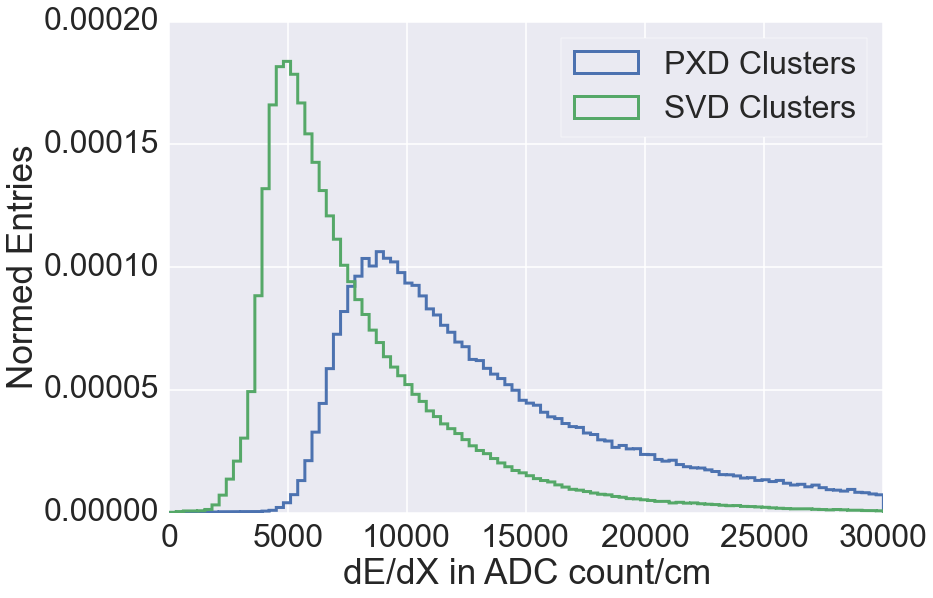
\includegraphics[width=0.48\linewidth]{figures/vxd/dEdXUncalibrated.png}
 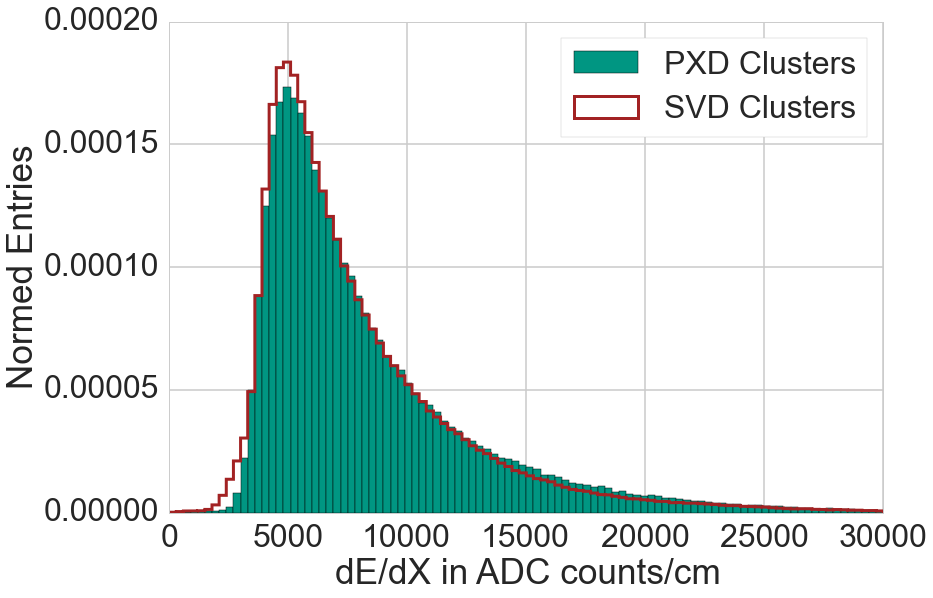
\includegraphics[width=0.48\linewidth]{figures/vxd/dEdXCalibrated.png}
 \caption{Distributions of the uncalibrated (left) and the calibrated (right) ADC counts of the PXD and SVD hits. Only clusters found by the VXD track finder are shown here.}
 \todo{Use ADC counts here!}
 \label{fig-adc-count}
\end{figure}




\subsection{Calculation of the path length in the clusters}
The \dedx value in every cluster can be calculated using the calibrated charge as described above and the length of the path the trajectory travels in the sensor region. There are five ways to calculate this path length implemented in the momentum estimation:
\begin{zlist}
 \item using the simulated MC information of the clusters,
 \item using the current trajectory parameters while fitting and a helix calculation,
 \item using the related MC trajectory at the origin,
 \item using the trajectory parameters estimated by the track finder without MC truth information,
 \item using the thickness of the cluster.
\end{zlist}

The different possibilities are ordered by their anticipated correctness. The two MC modes are only implemented for reference as they can obviously not be used in the later detector measurement. 

Besides the first and the last possibilities all modes rely on calculating the path length of a trajectory using only their helix parameters without any energy loss or material effects. This is done as follows:
\begin{zlist}
 \item Take the position of the cluster hit and calculate the distance to the beam line.
 \item Add and subtract half of the sensor thickness from this radius to gain an estimation of the start and the end radius of the sensor.
 \item Calculate the arc length from the perigee point to these two radii and from these arc lengths the distance between the two penetration points of the helix through the sensor using trigonometrical relations.
\end{zlist}

This procedure is correct for most of the cases but fails in some rare cases. Some examples are shown in figure \ref{fig-errors-in-path-length}. As it can be seen in the pictures errors in the calculation occur mainly for particles curling in the sensors. As the VXD sensors have only a very thin thickness the probability for such particles is very rare. Therefore these cases should not bias the momentum measurement much. Also as the calculation error can only occur in the most outer sensor touched by the particles all other senors give correct momentum estimations.

\begin{figure}
  \centering
  \todo{missing prictures}
  \caption{Exemplary cases of path length calculations. The correct path length is show in orange whereas the calculated one is shown in blue.}
  \label{fig-errors-in-path-length}
\end{figure}

In figure \ref{fig-pathlengths} the distribution of the correct path lengths from the simulated MC truth values is shown. As expected there are two peaks in the distribution - one for each hit type as the two types PXD and SVD have a different thickness. Most of the particles go more or less straight through the sensors. Deviations from the thickness come from curling particles. The fact that there are only few tracks with very high deviations from the thickness values verifies th claim that the helix calculation is wrong only for very rare cases.

The second subplot shows the distribution of the residuals of the other four path length calculations to these reference values as a violin plot.

\todo{Beschreibung!}

\begin{figure}
 \centering
%  \includegraphics{}
 \caption{The right plot shows the path length distribution as a result of the simulation. This distribution is used for reference in the right plot which shows the residuum distribution of the other path length calculation modes.}
\end{figure}


\subsection{Transformation function from dE/dX to momentum}


dEdX with calibration
Calculation of the function + calibration?
dEdX with p + fit on data + correction + q/p residdum etc.

- dedx with different pathlengths + delta
- fit result for landau (both plots),
- residuum, median + iqr function

\section{Incooperation in the helix fit}

MeasurementCreator, State On Plane -> TrackPoint

Results with fit, p value, iqr, median

Pictures:
- residuum, median + iqr function for different path length calculations
- p values